\section{MAESTRO Directory Structure}

\begin{figure}[h]
\centering
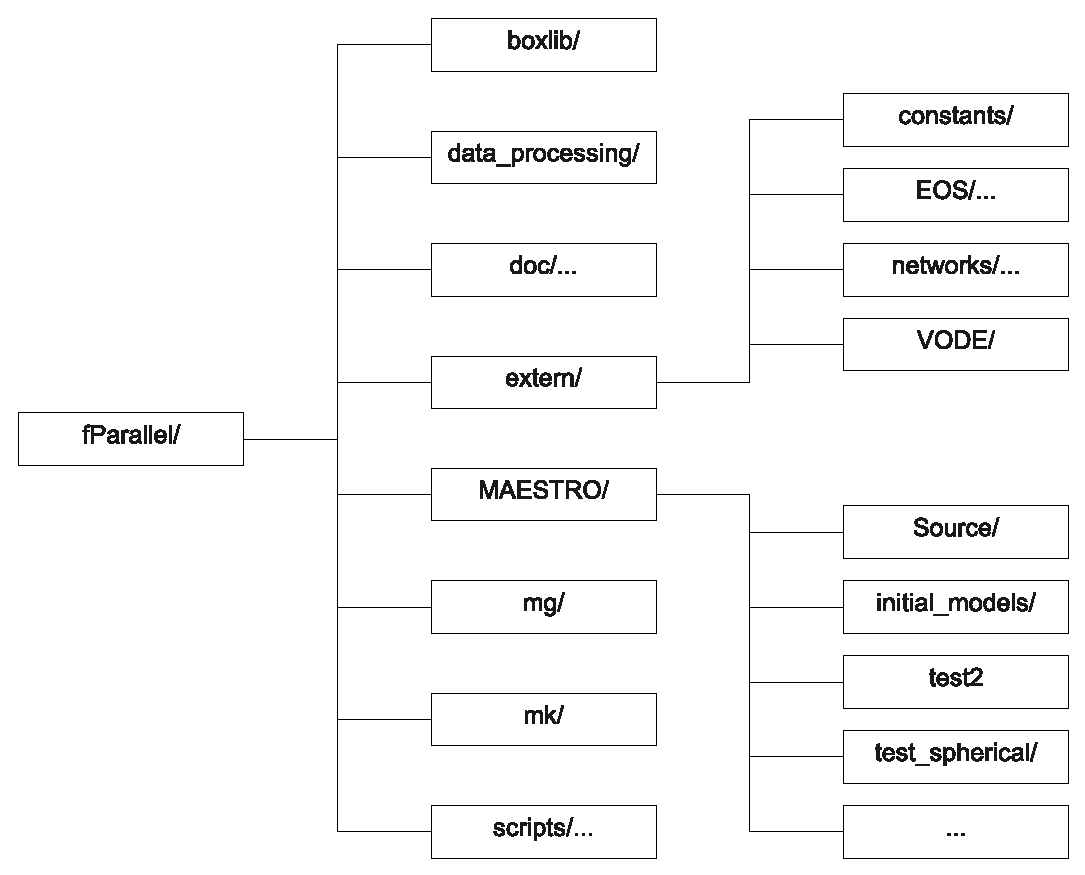
\includegraphics[width=5.0in]{\archfigpath/maestro_directory2}
\caption[MAESTRO directory structure]
{The basic MAESTRO directory structure}
\end{figure}

All the files needed to build MAESTRO are contained in the {\tt
fParallel} directory structure.  Briefly, the sub-directories
are:
\begin{itemize}
\item {\tt boxlib/} 

 BoxLib is a library for describing meshes consisting of a union
 of boxes.  The BoxLib modules define the basic datatypes used
 in MAESTRO.

\item {\tt data\_processing/}

 Simple Fortran-based analysis routines (e.g.\ extract a line from a
 multidimensional dataset) that operate on BoxLib datasets.

\item {\tt doc/}

 Documentation describing the basic algorithm.

\item {\tt extern/}

 External modules, like ODE integrators, equations of state, reaction
 networks

 Important subdirectories include:
 \begin{itemize}
 \item {\tt constants/}

 A simple module to define physical constants

 \item {\tt EOS/}

 A collection of various EOSes for use with the code.  The two
 important ones for MAESTRO are {\tt helmeos/} and {\tt
 gamma\_law\_general/}.

 \item {\tt networks/}

 Various reaction networks for MAESTRO problems.  In addition to
 providing a routine to evolve the nuclear species due to reactions,
 the networks also define the species that are advected by the code.

 \item {\tt VODE/}

 An integration package for ODEs.  At the moment, this is used 
 for integrating various reaction networks.
 
 \end{itemize}

\item {\tt MAESTRO/}

 The main MAESTRO algorithm files.  Here you will find the main driver,
 the advection routines, etc.

 Important directories under {\tt MAESTRO/} include:

 \begin{itemize}

 \item {\tt initial\_models}

   Several sub-directories containing routines to generate
   1D initial conditions in hydrostatic equilibrium for 
   mapping onto the MAESTRO grid.  See \S~\ref{sec:initial_models}
   for details.

 \item problem directories: {\tt test}, {\tt test2}, {\tt
   test\_spherical}, $\ldots$

   Each problem in MAESTRO gets it own subdirectory.  The {\tt
   GNUmakefile} includes the instructions on how to build the
   executable, including what modules in {\tt extern} are used.

   Any file that you place in a sub-directory here takes 
   precedence over a file of the same name in {\tt MAESTRO/}.
   This allows problems to have custom versions of the main
   MAESTRO routines (e.g.\ initial conditions via {\tt initdata.f90}.
   See \S~\ref{sec:makefile} for details on the build system.

 \end{itemize}

\item {\tt mg/}

  The multigrid solver.

\item {\tt mk/}

  The generic Makefiles that store the compilation flags for
  various platforms.

\item {\tt scripts/}

  Some simple scripts that are useful for building, running,
  maintaining MAESTRO.

\end{itemize}


\section{Getting Started}

In this section we describe some of the standard problems that come
with MAESTRO, how to run the code, some basic runtime parameters, and
how to look at the output.

\subsection{`Standard' Test Problems}

Different problems in MAESTRO are contained in individual
sub-directories under {\tt MAESTRO/}.  The {\tt GNUmakefile}
in each problem directory lists the components of {\tt MAESTRO}
that are used to build the executable.  Full details of the
{\tt GNUmakefile} can be found in \S~\ref{sec:adding_problems}.

Some of the test problems available are:
\begin{itemize}
\item {\tt flame} \\[-3mm]

The {\tt flame} problem models a planar laminar flame.  Initially cool
fuel and hot ash are put in pressure equilibrium.  Thermal diffusion
transfers heat to the fuel, driving a burning front.  This problem
does not use the traditional MAESTRO elliptic constraint, but
rather enforces $\nabla \cdot U = S$ (through the runtime parameter
{\tt do\_smallscale = T}) as discussed in \cite{SNe}.

\item {\tt spherical\_heat} \\[-3mm]

{\tt spherical\_heat} maps a spherical star (a Chandrasekhar-mass white
dwarf) onto the Cartesian domain and uses an external heat source to
cause the star to expand.  This is the 3-d analogue of the {\tt
  test\_basestate} unit test (see \S~\ref{sec:unit_tests}).  This
problem was discussed in \cite{multilevel}.

\item {\tt test2} \\[-3mm]

{\tt test2} places 3 hots spots in a plane-parallel atmosphere.
Burning makes these buoyant bubbles which role up.  This problem was
used in \cite{lowMach3} to compare with compressible solvers.

\item {\tt test\_convect} \\[-3mm]

{\tt test\_convect} drives convection through a plane-parallel
atmosphere using an externally-specified heat source.  This problem
was used to compare with compressible solvers in \cite{lowMach3}
and to test the multilevel algorithm in \cite{multilevel}.

\item {\tt test\_spherical} \\[-3mm]

{\tt test\_spherical} sets up an isentropically stratified star
and stirs it up with a random velocity field.  The low Mach number
constraint is replaced with the anelastic constraint (through
the {\tt beta\_type} runtime parameter).  Analytically, under
these conditions, the density of the star should not change.
This test problem was discussed in \cite{lowMach4}.

\end{itemize}


\subsection{Compiling and Running}

To build the MAESTRO executable, simply type `{\tt make}' in the
problem directory.  The executable will have a name like
{\tt main.Linux.Intel.exe}, where the specific parts of 
the name depend on the compilers and OS used.  Each problem
will have one or more inputs files (for example, {\tt test2/inputs\_2d})
which override the default values for one or more runtime parameters.
The code is run simply as:
\begin{verbatim}
  main.Linux.Intel.exe inputs_2d
\end{verbatim}
As the code runs, it will output both plotfiles and checkpoints.
By default, the plotfiles will be named {\tt plt}{\em nnnnn}, where
the number {\em nnnnn} is the timestep number when the file was
outputted.  Similarly, the checkpoints are named {\tt chk}{\em
  nnnnn}.  BoxLib plotfiles and checkpoints are actually directories,
with the data stored in subdirectories grouped by refinement level.
Details of the simulation (number of processors used, output date,
output directory, runtime parameter values, ...) are stored in
the {\tt job\_info} file in each plotfile directory.

A large number of runtime parameters affect the code's behavior.  Any
runtime parameter can be set either in the inputs file, as {\tt parameter
  = value} or on the command line by adding {\tt --parameter value} after
listing the inputs file on the command line.  A full list of runtime
parameters is detailed in \S~\ref{sec:runtime_parameters}.  Below we
outline the most common runtime parameters.

\subsection{Controlling Timestepping and Output}

Parameters that set the maximum time for the simulation to run
include:
\begin{itemize}
\item {\tt stop\_time} is the maximum simulation time, in seconds,
      to evolve the system for.

\item {\tt max\_step} is the maximum number of steps to take.
\end{itemize}

\noindent Parameters affecting the size of the timestep include:
\begin{itemize}
\item {\tt cflfac} is a multiplicative factor ({\tt $\le 1$}) 
      applied to the advective CFL timestep

\item {\tt init\_shrink} is the factor ({\tt $\le 1$}) by which to reduce 
      the initial timestep from the estimated first timestep.
\end{itemize}

\noindent Parameters affecting output and restart include:
\begin{itemize}

\item {\tt restart} tells MAESTRO to restart from a checkpoint.  The
      value of this parameter should be the file number to restart from.

\item {\tt plot\_int} is the number of steps to take between
  outputting a plotfile

\item {\tt plot\_deltat} is the simulation time to evolve between
  outputting a plotfile.  Note: to output only based on simulation
  time, set {\tt plot\_int = -1}.

\item {\tt check\_int} is the number of steps to take between
  outputting a checkpoint.

\end{itemize}

\subsection{Defining the Grid and Boundary Conditions}

Parameters that determine the spatial extent of the grid, 
the types of boundaries, and the number of computational cells include:
\begin{itemize}

\item {\tt max\_levs } is the maximum number of grid levels in the AMR
  hierarchy to us.  {\tt max\_levs = 1} indicates running with only a
  single level spanning the whole domain.

\item {\tt n\_cellx }, {\tt n\_celly }, {\tt n\_cellz } the size of
  base level in terms of number of cells, in the $x$, $y$, and $z$
  coordinate directions.

\item {\tt max\_grid\_size } the maximum extend of a grid, in any
  coordinate direction, as measured in terms of number of cells.

\item {\tt prob\_lo\_x }, {\tt prob\_lo\_y }, {\tt prob\_lo\_z } is
  the physical coordinate of the lower extent of the domain boundary
  in the $x$, $y$, and $z$ coordinate directions.

\item {\tt prob\_hi\_x }, {\tt prob\_hi\_y }, {\tt prob\_hi\_z } is
  the physical coordinate of the upper extent of the domain boundary
  in the $x$, $y$, and $z$ coordinate directions.

\item {\tt bcx\_lo }, {\tt bcy\_lo }, {\tt bcz\_lo }, 
      {\tt bcx\_hi }, {\tt bcy\_hi }, {\tt bcz\_hi } are the boundary
   condition types at the lower (`{\tt lo}') and upper (`{\tt hi}')
   domain boundaries in the $x$, $y$, and $z$ coordinate directions.
   The different types are set via integer flags noted below: 

   \begin{center}
   \begin{tabular}{ll}
   \hline
   BC type    & integer flag \\
   \hline
   periodic             & -1 \\
   inlet (user-defined) & 11 \\
   outlet               & 12 \\
   symmetry             & 13 \\
   slip wall            & 14 \\
   no-slip wall         & 15 \\
   \hline
   \end{tabular}
   \end{center}


\end{itemize}

Note that grid cells must be square, i.e. $\Delta x = \Delta y = \Delta z$
where $\Delta x$ on the base grid is computed as $({\tt prob\_hi\_x}
- {\tt prob\_lo\_x})/{\tt n\_cellx}$. 

\subsection{Refinement Criteria}

\subsection{Working with the Output}

Visualization and analysis are done with on the plotfiles.  A
number of in-house and externally developed tools can work 
with BoxLib-formatted plotfiles.


\subsubsection{\tt Amrvis}

{\tt Amrvis} is a visualization tool developed at LBL for 2- and 3-d
datasets which can plot slices through 3-d datasets as well as
volume-renderings.  It is distributed separately from the MAESTRO
distribution.


\subsubsection{{\tt data\_processing} scripts}

Several useful analysis scripts (written in Fortran 90) can be found
in {\tt fParallel/data\_processing}.  The {\tt GNUmakefile} there
needs to be edited to indicate which of the tools to build.  These
routines are described in \S~\ref{sec:analysis}.


\subsubsection{VisIt}

VisIt is a powerful, DOE-supported visualization tool for 2- and 3-d
datasets.  It can do contouring, volume rendering, streamlines, ...\
directly from BoxLib plotfiles (to open a plotfile in VisIt, point to
the {\tt Header} file inside the plotfile directory.  Details on
visit can be found at {\tt https://wci.llnl.gov/codes/visit/home.html}\,.



\subsection{Unit Tests}

\label{sec:unit_tests}

In addition to the problems descibed above which use the full
capabilities of MAESTRO, there are a number of unit tests that
exercise only specific components of the MAESTRO solvers.  The
tests have their own drivers (a custom {\tt varden.f90}) that
initialize only the data needed for the specific test and call
specific MAESTRO routines directly.

\begin{itemize}
\item {\tt test\_advect} \\[-3mm]

  This test initializes a Gaussian density field (no other scalar
  quantities are used) and a uniform velocity field in any one of the
  coordinate directions.  The Gaussian profile is advected through
  the period domain exactly once and the error in the density profile
  (L2 norm) is computed.  The driver for this problem does this 
  for every dimension twice (once with a positive velocity and once
  with a negative velocity).  After all coordinate directions are 
  tested, the norms are compared to ensure that the error does
  not show any directional bias.


\item {\tt test\_average} \\[-3mm]

  This test initializes a 1-d radial base state quantity with a
  Gaussian distribution, maps it into the 3-d domain (assuming a
  spherical geometry) using the routines provided by the {\tt
    fill\_3d\_module} module, and then calls {\tt average} to put it
  back onto a 1-d radial array.  This way we test the accuracy of our
  procedure to map between the 1-d radial and 3-d Cartesian states.
  The output from this test was described in detail in
  \cite{multilevel}.

\item {\tt test\_basestate} \\[-3mm]

  This test initializes the base state to contain a hydrostatic
  model and then evolves the state with heating to watch the 
  hydrostatic adjustment of the atmosphere.  In particular,
  the base state velocity, $w_0$, is computed in response to 
  the heating and this is used to advect the base state density
  and compute the new pressure, $p_0$.  An early version of 
  this routine was used for the plane-parallel expansion test
  in \cite{lowMach2}.  This version of the test was also shown
  for a spherical, self-gravitating star in \cite{multilevel}.

  
\item {\tt test\_diffusion}

  This test initializes a Gaussian temperature profile and calls
  the thermal diffusion routines in MAESTRO to evolve the state 
  considering only diffusion.  The driver estimates a timestep
  based on the explicit thermal diffusion timescale and loops
  over calls to the thermal diffusion solver.  A Gaussian remains
  Gaussian when diffusing, so an explicit error can be computed
  by comparing to the analytic solution.  This test is 
  described in \cite{xrb}.

\end{itemize}


\section{Adding A New Problem}
\label{sec:adding_problems}

Different MAESTRO problems are defined in subdirectories under
{\tt MAESTRO/}.  To add a problem, start by creating a new
sub-directory---this is where you will compile your problem and
store all the problem-specific files.

The minimum requirement to
define a new problem would be a {\tt GNUmakefile} which describes how
to build the application and an input file which lists the runtime
parameters.  The problem-specific executable is built in the problem
directory by typing {\tt make}.  Source files are found automatically
by searching the directories listed in the {\tt GNUmakefile}.
Customised versions of any source files placed in the problem-directory
override those with the same name found elsewhere.  Any unique
source files (and not simply a custom version of a file found
elsewhere) needs to be listed in a file call {\tt GPackage.mak}
in the problem-directory.

\subsection{The {\tt GNUmakefile}}

\label{sec:makefile}

A basic {\tt GNUmakefile} begins with:
\begin{verbatim}
  NDEBUG := t
  MPI    :=
  OMP    :=
\end{verbatim}
Here, {\tt NDEBUG} is true is we are building an optimized executable.
Otherwise, the debug version is built---this typically uses less
optimization and adds various runtime checks through compiler flags.
{\tt MPI} and {\tt OMP} are set to true if we want to use either MPI
or OpenMP for parallelization.

The MAESTRO build system knows what options to use for various
compiler families.  The {\tt COMP} flag specifies which compiler to
us.  Allowed values include {\tt Intel}, {\tt gfortran}, {\tt PGI},
and {\tt PathScale}.  The specific details of these choices are
defined in the {\tt MAESTRO/mk/} directory.
\begin{verbatim}
  COMP := Intel
  MKVERBOSE := t
\end{verbatim}
{\tt MKVERBOSE} set to true will echo the build commands to the
terminal as the are executed.

The next set of lines tell the build system where to look for source
files.  A MAESTRO application is built from several pacakges (the
multigrid solver, an EOS, a reaction network, etc.).  
\begin{verbatim}
  FPARALLEL := ../..

  include $(FPARALLEL)/mk/GMakedefs.mak

  Fmdirs := boxlib \
            mg \
            MAESTRO \
            extern/EOS/helmeos \
            extern/EOS/conducteos \
            extern/constants \
            extern/networks/ignition \
            extern/VODE

  Fmincludes := extern/EOS/helmeos
\end{verbatim}
The {\tt FPARALLEL} variable should point to the top-level directory
of the source tree (i.e.\ {\tt fParallel/}).  Next we include the
compiler definitions, {\tt mk/GMakedefs.mak}.  The {\tt Fmdirs}
variable lists the individual directories in the {\tt fParallel/}
source tree that are used to build the problem.  Generally, one does
not need to include the problem directory itself, unless there are
unique source files found there, described in a {\tt GPackage.mak}
file.  The build system will attempt to build all of the files listed
in the various {\tt GPackage.mak} files found in the {\tt Fmdirs}
directories.  Furthermore, {\tt Fmdirs} will be will be added to the
{\tt make} {\tt VPATH}, which is the list of directories to search for
source files.  The problem directory will always be put first in the
{\tt VPATH}, so any source files placed there override those with the
same name found elsewhere in the source tree.  The {\tt Fmincludes}
variable lists all those directories that contain include files that
are inserted into the Fortran source at compile time via the {\tt
  include} statement.  Presently, the only instance of this is with
the Helmholtz general equation of state found in {\tt
  extern/EOS/helmeos/}.

Runtime parameters listed in the {\tt MAESTRO/\_parameters} file are
parsed at compile time and the file {\tt probin.f90} is written and
compiled.  This is a Fortran module that holds the values of the
runtime parameters and makes them available to any routine.  The
variable {\tt PROBIN\_PARAMETERS} should list all of the files that
contain runtime parameters for the current problem.  You must always
include the main {\tt ../\_parameters} file (i.e.\ {\tt
  MAESTRO/\_parameters}).  Sometimes a problem defines their own
runtime parameters (see \S~\ref{sec:def_runtime_param}), in which
case, its parameter file should also appear in {\tt
  PROBIN\_PARAMETERS}.
\begin{verbatim}
  PROBIN_PARAMETERS := ../_parameters
\end{verbatim}

The final lines in the {\tt GNUmakefile} include the rules to actually
build the executable.
\begin{verbatim}
  include $(FPARALLEL)/MAESTRO/GMaestro.mak
  include $(FPARALLEL)/mk/GMakerules.mak
\end{verbatim}

As mentioned above, any source files placed in the problem directory
override a files with the same name found elsewhere in the source
tree.  This allows you to create a problem-specific version of any
routine.  Source files that are unique to this problem (i.e.\ there is
no file with the same name elsewhere in the source tree) need to be
listed in a file {\tt GPackage.mak} in the problem directory.


\subsection{Defining Runtime Parameters}

\label{sec:def_runtime_param}

The runtime parameters for the core MAESTRO algorithm are listed
in {\tt MAESTRO/\_parameters}.  That file is parsed at compile-time
by the {\tt MAESTRO/write\_probin.py} script
(along with any other parameter files listed in the {\tt PROBIN\_PARAMETERS}
variable in the {GNUmakefile}, see \S \ref{sec:makefile}).  The script
outputs the {\tt probin.f90} source file.  Each line
in the {\tt \_parameters} file has the form: 
\vskip 3mm
{\em parameter} \hskip 10em  {\em data-type} \hskip 10em  {\em value} 
\vskip 3mm
\noindent where {\em parameter} is the name of the runtime parameter,
{\em data-type} is one of \{{\tt character}, {\tt real}, {\tt
  integer}, {\tt logical}\}, and the {\em value} specifies the default
value for the runtime parameter.  Comments are indicated by a `{\tt
  \#}' character and a used to produce documentation about the
available runtime parameters.

At runtime, the default values for the parameters can be overridden
either through the inputs file (by adding a line of the form: {\tt
  parameter = value}) or through a command-line argument (taking the
form: {\tt --parameter value}).  The {\tt probin\_module} makes the
values of the runtime parameters available to the various functions
in the code (see \S~\ref{sec:probin}).

Problem-specify runtime parameters should be defined in the
problem-directory in a file called {\tt
  \_parameters}\{{\em.problem-name}\}.  This file should be added
to the {\tt PROBIN\_PARAMETERS} variable in the {\tt GNUmakefile}.



\subsection{Preparing the Initial Model}

\label{sec:initial_models}

MAESTRO models subsonic flows that are in hydrostatic equilibrium.
The solution in MAESTRO is broken up into a 1-d base state and the 2-
or 3-d full state.  The job of the 1-d base state in the algorithm is
to represent the hydrostatic structure.  The full, Cartesian state
carries the departures from hydrostatic equilibrium.  The underlying
formulation of the low Mach number equations assumes that the base
state is in hydrostatic equilibrium.  At the start of a simulation,
the initial model is read in and taken as the base state.  Therefore,
any initial model needs to already be in hydrostatic equilibrium.

The routines in {\tt MAESTRO/initial\_model/} prepare an initial model
for MAESTRO.  There are two types of routines here, the first type
take an existing 1-d initial model produced somewhere else (e.g.\ a
1-d stellar evolution code), and and map it onto a uniform grid, at
the desired resolution, using the equation of state in MAESTRO, and
using MAESTRO's discretization of hydrostatic equilibrium.  The second
type generate the initial model internally, by integrating the
condition of hydrostatic equilibrium together with a simplifying
assumption on the energy (e.g. isothermal or isentropic).  In
both cases hydrostatic equilibrium is enforced as:
\begin{equation}
\frac{p_{i+1} - p_i}{\Delta r} = \frac{1}{2} (\rho_i + \rho_{i+1})
g_{i+1/2}
\end{equation}

The {\tt toy\_atm} example provides a simple approximation for a thin
(plane-parallel) convectively-unstable accreted layer on the surface
of a star.  This can be used as the starting point for a more complex
model.  Further details on the initial model routines can be 
found in \S~\ref{sec:initial_models_main}.



\section{BoxLib Data Structures}

MAESTRO's gridding is handled by the BoxLib library.  The underlying
idea in BoxLib is to allow for adaptive mesh refinement (AMR)---different
regions of the domain can have different spatial resolutions.  The
domain is broken into boxes.  At the coarsest (base) level of
refinement, the entire computational domain is covered, either by one
box or broken across many boxes.  Higher levels of refinement have
finer zones (typically $2\times$).  Only a portion of the domain may
be covered by the higher levels of refinement.  \MarginPar{Nesting?}
For parallel computations, the boxes are spread across processors, in
a fashion designed to put roughly equal amounts of work on each
processor (load balancing).

On a grid, the data can be stored at cell-centers, on a face/edge, or
on the corners.  In BoxLib, data that is on an edge is termed `nodal'
in that direction (see Figure~\ref{fig:dataloc}).  Data that is on the
corners is nodal in all spatial directions.  In MAESTRO, the state
data (density, enthalpy, velocity, $\ldots$) is generally
cell-centered.  Fluxes are nodal in the direction they represent.
A few quantities are nodal in all directions (e.g.\ $\phi$ used in
the final velocity projection).

\begin{figure}[h]
\centering
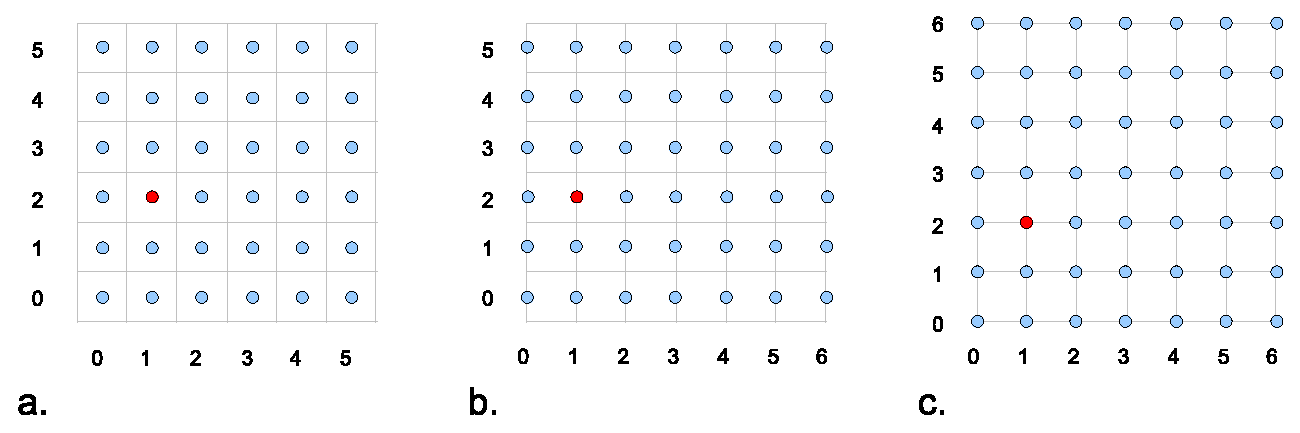
\includegraphics[width=6.5in]{\archfigpath/data_loc2}
\caption[Data-centerings on the grid]
  {\label{fig:dataloc} Some of the different data-centerings:
  (a) cell-centered, (b) nodal in the $x$-direction, and (c) nodal in
  both the $x$- and $y$-directions.  Note that for nodal data, the
  integer index corresponds to the lower boundary in that direction.
  In each of these centerings, the red point has the same indices:\ (1,2).
  Not shown is the case where data is nodal in the $y$-direction only.}
\end{figure}



To simplify the description of the underlying AMR grid, BoxLib
provides a number of Fortran types.  We briefly summarize the major
data types below.


\subsection{\boxtype}

A \boxtype\ is simply a rectangular domain in space.  Note that boxes
do not hold the state data themselves.  The datatype for a
\boxtype\ is
\begin{verbatim}
  type box
     integer :: dim  = 0
     integer :: lo(MAX_SPACEDIM) =  Huge(1)
     integer :: hi(MAX_SPACEDIM) = -Huge(1)
  end type box
\end{verbatim}

\noindent Here:
\begin{itemize}
\item {\tt dim} is the dimensionality of the data
\item {\tt lo} is the index of the lower bound of the box
\item {\tt hi} is the index of the upper bound of the box
\end{itemize}


\begin{figure}[h]
\centering
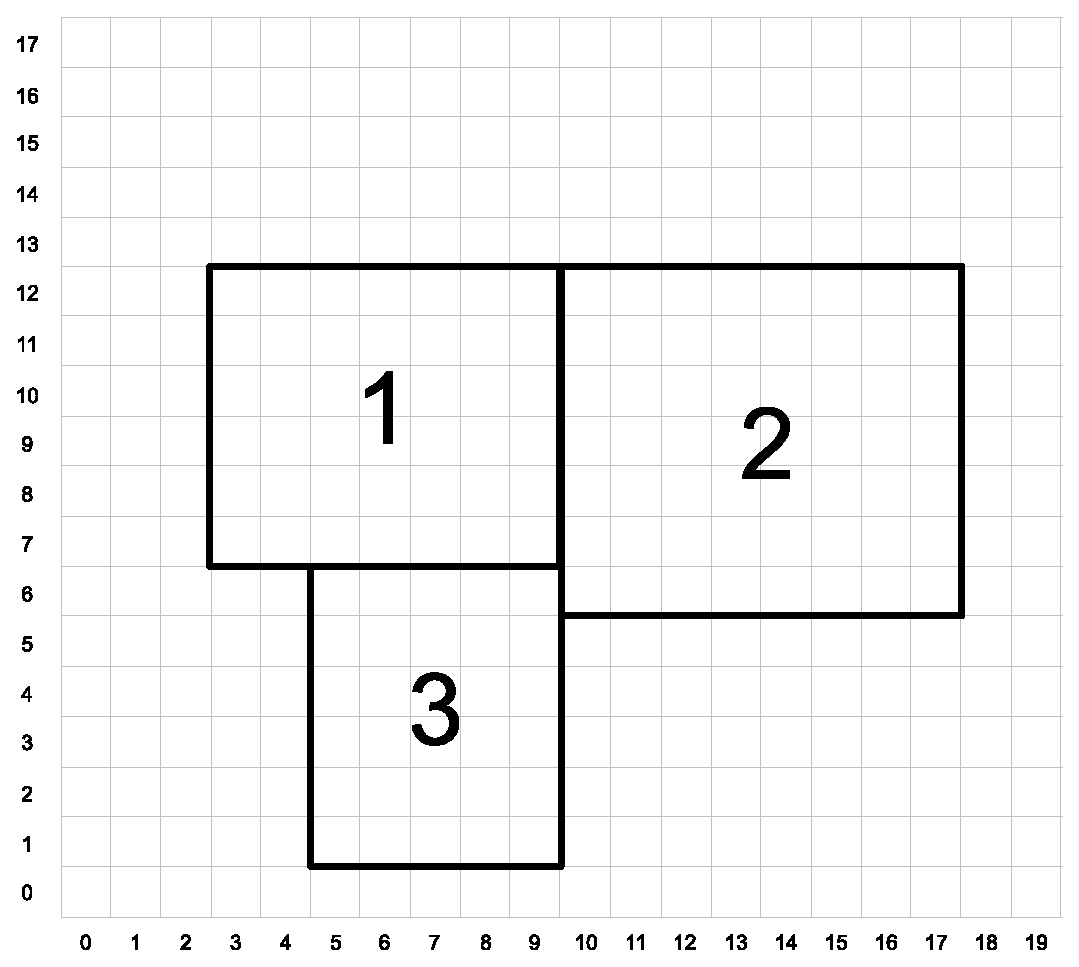
\includegraphics[width=4.0in]{\archfigpath/index_grid2}
\caption[Single-level grid structure]
{\label{fig:boxes} Three boxes that comprise a single level.  At this
  resolution, the domain is 20$\times$18 zones.  Note that the
  indexing in BoxLib starts with $0$.}
\end{figure}


The computational domain is divided into boxes.  The collection of
boxes with the same resolution comprise a level.
Figure~\ref{fig:boxes} shows three boxes in the same level of
refinement.  The position of the boxes is with respect to a global
index space at that level.  For example, box 1 in the figure has {\tt
  lo} = (3,7) and {\tt hi} = (9,12).


\subsubsection{Common Operations on a \boxtype}

For a \boxtype\ declared as:
\begin{verbatim}
  type(box) :: mybox
\end{verbatim}

\begin{itemize}

\item {\tt lo = lwb(mybox)} returns an array, {\tt lo(dm)}, with
     the box lower bounds

\item {\tt hi = upb(mybox)} returns an array, {\tt hi(dm)}, with
     the box upper bounds

\end{itemize}



\subsection{\fab}

A \fab\ is a ``Fortran Array Box''.  It contains the state data in a
multidimensional array and several \boxtype-types to describe where in
index-space it lives.  The datatype of a \fab\ is
\begin{verbatim}
  type fab
     integer   :: dim = 0
     type(box) :: bx
     type(box) :: pbx
     type(box) :: ibx
     integer   :: nc = 1
     real(kind = dp_t), pointer, dimension(:,:,:,:) :: p => Null()
  end type fab
\end{verbatim}
 
\noindent Here:
\begin{itemize}
\item {\tt dim} is the dimensionality of the data
\item {\tt bx} is a \boxtype\ describing the index space for which this \fab\ is defined
\item {\tt ibx} is a \boxtype\ that describes the index range of the valid data
  for the \fab.  This differes from {\tt bx} when the box is nodal in one or more 
  directions.
\item {\tt pbx} is a \boxtype\ that extends {\tt ibx} to include
  any ghostcells, or equivalently, the physical box for the \fab\
\item {\tt nc} is the number of components (how many variables at  
  each grid location)
\item {\tt p} is a pointer to the data, in this case double precision
  ({\tt kind=dp\_t}).  Other \fab\ types exists for other Fortran
  data types.
\end{itemize}


Note that all state data is stored in a four-dimensional array,
{\tt (nx,ny,nz,nc)} in size, regardless of the dimensionality of the
problem.  For 2D problems, {\tt nz=1}.

In MAESTRO, we don't usually deal with \fab s alone, but rather
through \multifab s, described next.

\subsection{\multifab}

A \multifab\ is a collection of \fab s at the same level of
refinement.  The data type of a \multifab\ is:
\begin{verbatim}
  type multifab
     integer :: dim = 0
     integer :: nboxes = 0
     integer :: nc = 1
     integer :: ng = 0
     logical, pointer :: nodal(:) => Null()
     type(layout) :: la
     type(fab), pointer :: fbs(:) => Null()
  end type multifab
\end{verbatim}




\subsection{\boxarray}

A \boxarray\ is an array of boxes

\subsection{\mlboxarray}

A \mlboxarray\ is a collection of \boxarray s at different levels of
refinement.

\subsection{\mllayout}


\subsection{\bctower}


\section{MAESTRO Data Organization}

The state of the star in MAESTRO is described by both a
multidimensional state and the 1D base state.  The full
multidimensional state is stored in \multifab s while the base state
is simply stored in Fortran arrays.  Here we describe the
major MAESTRO data-structures.

\subsection{`{\tt s}' \multifab s (fluid state)}

The fluid state (density, enthalpy, species) are stored together in a
cell-centered multi-component \multifab, typically named {\tt sold},
{\tt s1}, {\tt s2}, or {\tt snew} (depending on which time-level it
represents).  The enthalpy is stored as $(\rho h)$, and the species
are stored as partial-densities $(\rho X_k)$.

Individual state variables should be indexed using the integer keys provided 
by the {\tt variables} module (see \S \ref{sec:variables_module}).  For example,
the integer {\tt rho\_comp} will always refer to the density component of the state.


\subsection{`{\tt u}' \multifab s (fluid velocity)}

The fluid velocity at time-levels $n$ and $n+1$ is stored in
a cell-centered multi-component \multifab, typically named
{\tt uold} or {\tt unew}.  Here the {\tt dm}
components correspond to each coordinate direction.

\subsection{{\tt umac} (the MAC velocity)}

In creating the advective fluxes, we need the time-centered velocity
through the faces of the zone---the $x$-velocity on the $x$-edges, the
$y$-velocity on the $y$-edges, etc.\ (see figure~\ref{fig:mac}).  This
type of velocity discretization is termed the MAC velocity (after the
``marker-and-cell'' method for free boundaries in incompressible
flows \cite{harlowwelch:1965}).



\begin{figure}[h]
\centering
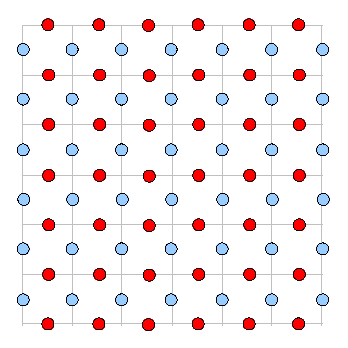
\includegraphics[width=2.5in]{\archfigpath/mac2}
\hspace{0.1in}
\begin{minipage}[b]{3.8in}
\caption[The MAC grid]
{\label{fig:mac} The MAC grid for the velocity.  
Here the $x$-velocity is on the $x$-edges (shown as the 
blue points) and the $y$-velocity is on the $y$-edges
(shown as the red points).
}\ \\
\end{minipage}
\end{figure}

The MAC velocities are allocated at each level of refinement, {\tt n},
by making a \multifab\ array where each of the {\tt dm} components is
nodal in its respective direction:
\begin{verbatim}
  type(multifab) :: umac(dm)

  do comp=1,dm
     call multifab_build(umac(n,comp), mla%la(n),1,1, &
                         nodal=edge_nodal_flag(comp,:))
  enddo
\end{verbatim}



\subsection{Base State Arrays}

The base state is defined by $\rho_0$, $p_0$, and $w_0$.  There is no
base state composition.  Other arrays are defined as needed, such as
$h_0$, the base state enthalpy.

\subsection{Other Quantities}


\section{MAESTRO Helper Modules}

A number of MAESTRO modules appear frequently throughout the source.
Below, we describe some of the more common functionality of the most
popular modules.

\subsection{\tt average}

\subsection{{\tt eos\_module}}

The {\tt eos\_module} provides the interface to the equation of 
state to connect the state variables thermodynamically.  It 
gets the information about the fluid species from the {\tt network}
module (for example, the atomic number, $Z$, and atomic weight, $A$,
of the nuclei).

Presently there are 2 equations of state that work with MAESTRO:
\begin{itemize}
\item {\tt extern/EOS/helmeos/} represents a general stellar equation 
      of state, consisting of nuclei (as an ideal gas), radiation,
      and electrons (with arbitrary degeneracy and degree of relativity).
      This equation of state is that described in \cite{timmes_eos}.

\item {\tt extern/EOS/gamma\_law\_general} assumes an ideal gas with a mixed 
     composition and a constant ratio of specific heats, $\gamma$:
      \begin{equation}
      p = \rho e (\gamma - 1) = \frac{\rho k_B T}{\mu m_p} 
      \end{equation}
     where $k_B$ is Boltzmann's constant and $m_p$ is the mass of the
     proton.
     The mean molecular weight, $\mu$, is computed assuming 
     electrically neutral atoms:
     \begin{equation}
     \mu = \left ( \sum_k \frac{X_k}{A_k} \right )^{-1}
     \end{equation}
     An option in the source code itself exists for treating the
     species as fully-ionized, but there is no runtime-parameter to
     make this switch.
\end{itemize}

eos module variables

eos input types


\subsection{{\tt fill\_3d\_module}}

\subsection{{\tt geometry}}

\subsection{{\tt network}}

The {\tt network} module defines the number species advected by the
code ({\tt nspec}), their ordering, and gives their basic properties
(like atomic number, $Z$, and atomic mass, $A$).  All MAESTRO problems
require a {\tt network} module, even if there are no reactions
modeled.  Many different reaction modules (containing different sets
of isotopes) exist in {\tt extern/networks}.  The particular network
used by a problem is defined in the problem's {\tt GNUmakefile}.

To find the location of a particular species (for instance, ``carbon-12'')
in the allowed range of {\tt 1:nspec}, you do the following query:
\begin{verbatim}
  ic12 = network_species_index("carbon-12")
\end{verbatim}
If the resulting index is {\tt -1}, then the requested species was not
found.

\subsection{{\tt probin\_module}}

\label{sec:probin}

{\tt probin\_module} provides access to the runtime parameters.
The runtime parameters appear simply as module variables.  To get the 
value of a parameter, one simply needs to `{\tt use probin\_module}'.
The preferred method is to add the `{\tt only}' clause to the
{\tt use} statement and explicitly list only those parameters that
are used in the routine.  Defining new runtime parameters is
described in \S~\ref{sec:def_runtime_param}.

\subsection{{\tt variables}}

\label{sec:variables_module}

The {\tt variables} module provides integer keys to index the state
multifabs and other arrays dealing with the scalar quantities.  The
most commonly used keys are are:

\begin{center}
\begin{tabular}{ll}
\hline
{\tt rho\_comp}  & density \\
{\tt rhoh\_comp} & density $\times$ specific enthalpy, $(\rho h)$ \\
{\tt spec\_comp} & first species partial density, $(\rho X_1)$ \\
{\tt temp\_comp} & temperature \\
\hline
\end{tabular}
\end{center}

The species indices are contiguous in the state array, spanning {\tt spec\_comp:spec\_comp-1+nspec}.
To find a particular species, a query can be made through the {\tt
  network} module, such as:
\begin{verbatim}
  ic12 = network_species_index("carbon-12")
\end{verbatim}
and then the \fab\ can be indexed using {\tt spec\_comp-1+ic12} to
get ``carbon-12''.
The {\tt variables} module also provides keys for the plotfile
variables and boundary condition types.


\section{BoxLib Helper Modules}

There are a large number of modules in {\tt boxlib/} that provide
the core functionality for managing grids.  Here we describe
the most popular such modules.


\subsection{{\tt bl\_types}}

\subsection{{\tt bl\_constants}}

\subsection{{\tt parallel}}

\section{Example: Accessing State Data}

In MAESTRO, the state data is stored in a multifab array (the array
index refers to the AMR level).  A typical way to extract the state data
array looks like:

\begin{verbatim}
  subroutine example(s,dx,dt)

    use bl_types
    use multifab_module
    use geometry, only: dm, nlevs
    use variables, only: rho_comp
\end{verbatim}

\noindent Here, the {\tt bl\_types} and {\tt multifab\_module} modules
bring in the basic BoxLib data types. Specifically, here, {\tt
bl\_types} defines {\tt dp\_t} which is the {\tt kind} used for
declaring double precision data, and {\tt multifab\_module} defines
the \multifab\ data type.  The {\tt geometry} module is a MAESTRO
module that provides the dimensionality ({\tt dm}) and the number of 
levels ({\tt nlevs}).  The {\tt variables} module is a MAESTRO
module that provides integer keys for indexing the state arrays.  In
this case the integer {\tt rho\_comp} refers to the location in the
state array corresponding to density.

\begin{verbatim}
    type(multifab) , intent(inout) :: s(:)
    real(kind=dp_t), intent(in   ) :: dx(:,:),dt
\end{verbatim}

\noindent Next we declare the subroutine arguments.  Here, {\tt s(:)}
is our \multifab\ array that holds the state data.  The array index
in {\tt s} refers to the AMR level.

\begin{verbatim}
    ! Local variables
    real(kind=dp_t), pointer :: sp(:,:,:,:)
    integer :: i,n,ng_sp
    integer :: lo(dm),hi(dm)
\end{verbatim}

\noindent Amongst the local variables we define here are a pointer,
{\tt sp}, that will point to a single \fab\ from the
\multifab\ {\tt s}.

\begin{verbatim}
    ng_sp = s(1)%ng
\end{verbatim}

\noindent Here we get the number of ghostcells for this particular
\multifab.  This will be needed to access the data stored in the
\fab s.  Note that all levels in a \multifab\ will have the same
number of ghostcells, so we can use {\tt s(1)} here.

\begin{verbatim}
    do n=1,nlevs
       do i = 1, s(n)%nboxes
\end{verbatim}

\noindent To access the data, we loop over all the levels, and
all the boxes in the given level.  {\tt s(n)\%nboxes} is simply
the number of boxes in level {\tt n}.

\begin{verbatim}
          if ( multifab_remote(s(n), i) ) cycle
          sp => dataptr(s(n), i)
          lo =  lwb(get_box(s(n), i))
          hi =  upb(get_box(s(n), i))
\end{verbatim}

\noindent For parallel runs, there is no guarantee that the particular
box is on the current processor.  The function {\tt multifab\_remote}
returns {\tt .true.} if the box is off-processor, in which case, we 
simply skip to the next box.

The actual data array is accessed through the {\tt dataptr} function,
which takes a \multifab\ (in this case, {\tt s(n)}) and the index of
the \boxtype\ ({\tt i}) we want.  {\tt sp} is always four-dimensional:
3 spatial dimensions and 1 for the components.

Finally, the index bounds of the box (just the data, not the ghostcells) are 
stored in the {\tt dm}-dimensional arrays {\tt lo} and {\tt hi}

\begin{verbatim}
          select case (dm)
          case (2)
             call example_2d(sp(:,:,1,rho_comp),ng_sp,lo,hi,dx(n,:),dt)
          case (3)
             call example_3d(sp(:,:,:,rho_comp),ng_sp,lo,hi,dx(n,:),dt)
          end select
       enddo    ! end loop over boxes

    enddo    ! end loop over levels

  end subroutine example
\end{verbatim}

\noindent Finally, in this example, we call either the function
{\tt example\_2d} for two-dimensional data or {\tt example\_3d}
for three-dimensional data.  Note that in the two-dimensional
case, we index the data as {\tt sp(:,:,1,rho\_comp)}.  Here a
`{\tt 1}' is used as the `z'-coordinate spatial index, since this
is a 2D problem, and the density component of the state is selected
(using the integer key {\tt rho\_comp}).

This routine will be supplimented with {\tt example\_2d} and {\tt
example\_3d}, which actually operate on the data.  The form of 
these functions is:

\begin{verbatim}
  subroutine example_2d(density,ng_sp,lo,hi,dx,dt)

    use bl_constants_module
    use probin_module, only: prob_lo

    integer        , intent(in) :: lo(:),hi(:), ng_sp
    real(kind=dp_t), intent(in) :: density(lo(1)-ng_sp:,lo(2)-ng_sp:)
    real(kind=dp_t), intent(in) :: dx(:),dt

    integer         :: i, j
    real(kind=dp_t) :: x, y

    do j = lo(2), hi(2)
       y = prob_lo(2) + (dble(j) + HALF)*dx(2)

       do i = lo(1), hi(1)
          x = prob_lo(1) + (dble(i) + HALF)*dx(1)

          ! operate on density(i,j)
          ! ...

       enddo
    enddo

  end subroutine example_2d
\end{verbatim}

\noindent In this function, the bounds of the {\tt density} array
take into account the {\tt ng\_sp} ghostcells.  The {\tt j} and {\tt i}
loops loop over all the valid zones.  Coordinate information is 
computed from {\tt dx} and {\tt prob\_lo} which is the physical
lower bound of the domain.  {\tt bl\_constants\_module} declares
useful double-precision constants, like {\tt HALF} (0.5).

The three-dimensional case is similar, with the {\tt density} array
declared as 
\begin{verbatim}
  density(lo(1)-ng_sp:,lo(2)-ng_sp:,lo(3)-ng_sp)
\end{verbatim}
and an additional loop over the `z' coordinate (from {\tt lo(3)} to
{\tt hi(3)}).

\section{Working with Multifabs}

need to describe the routines for adding two multifabs, subtracting,
etc. and norm, etc.

\section{Filling Ghostcells}


\section{Boundary Conditions}


\section{Multigrid}


